\documentclass[border=5pt]{standalone}
\usepackage{graphicx}
\usepackage{tikz}
\usepackage{pgfplots}
\usetikzlibrary{calc}
\usetikzlibrary{patterns}
\usetikzlibrary{decorations.text}
\usetikzlibrary{shapes,snakes}
\usetikzlibrary{arrows.meta}
\usetikzlibrary{decorations}

\pgfdeclaredecoration{dashsoliddouble}{initial}{
  \state{initial}[width=\pgfdecoratedinputsegmentlength]{
    \pgfmathsetlengthmacro\lw{.3pt+.5\pgflinewidth}
    \begin{pgfscope}
      \pgfpathmoveto{\pgfpoint{0pt}{\lw}}%
      \pgfpathlineto{\pgfpoint{\pgfdecoratedinputsegmentlength}{\lw}}%
      \pgfmathtruncatemacro\dashnum{%
        round((\pgfdecoratedinputsegmentlength-3pt)/6pt)
      }
      \pgfmathsetmacro\dashscale{%
        \pgfdecoratedinputsegmentlength/(\dashnum*6pt + 3pt)
      }
      \pgfmathsetlengthmacro\dashunit{3pt*\dashscale}
      \pgfsetdash{{\dashunit}{\dashunit}}{0pt}
      \pgfusepath{stroke}
      \pgfsetdash{}{0pt}
      \pgfpathmoveto{\pgfpoint{0pt}{-\lw}}%
      \pgfpathlineto{\pgfpoint{\pgfdecoratedinputsegmentlength}{-\lw}}%     
      \pgfusepath{stroke}
    \end{pgfscope}
  }
}




\renewcommand\familydefault{\sfdefault}

\tikzset{
dot/.style = {circle, fill, minimum size=#1,
              inner sep=0pt, outer sep=0pt},
dot/.default = 6pt % size of the circle diameter 
}

\begin{document}
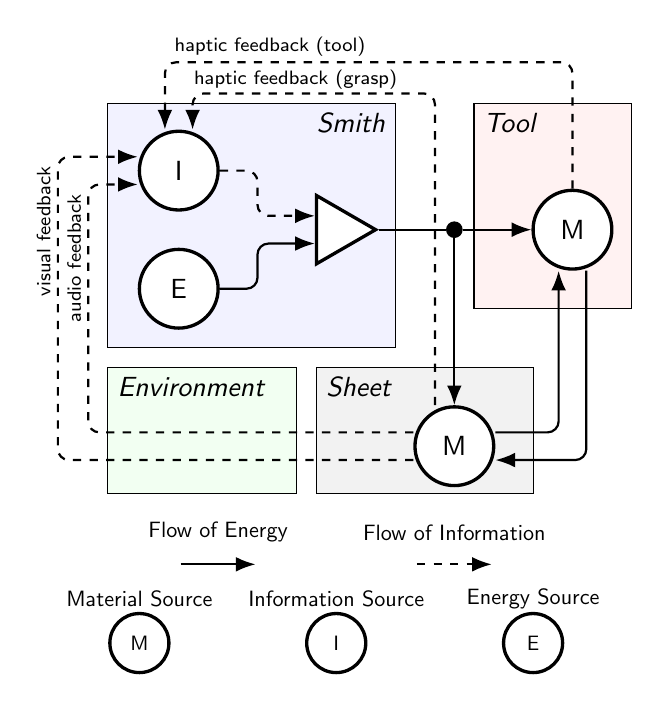
\begin{tikzpicture}[S/.style={circle, draw=black, fill=white!5, very thick, minimum size=10mm},
T/.style={regular polygon, regular polygon sides=3,shape border rotate=270, draw=black, fill=white, very thick, minimum size=10mm},
lI/.style={rounded corners,dashed,thick,-{Latex[length=2.5mm]}},
li/.style={rounded corners,dashed,thick},
lE/.style={rounded corners,thick,-{Latex[length=2.5mm]}}]
%
%\draw[help lines, color=gray!30, dashed] (0,0) grid (40,25);
%\draw[->,ultra thick] (0,0)--(20,0) node[below]{y};
%\draw[->,ultra thick] (0,0)--(0,10) node[above]{x};
%

\filldraw[fill=blue!5!white, draw=black] (9.1,7.75) rectangle (12.75,10.85);
\node[anchor=north east] at (12.75,10.85) {\textit{Smith}};

\filldraw[fill=red!5!white, draw=black] (13.75,8.25) rectangle (15.75,10.85);
\node[anchor=north west] at (13.75,10.85) {\textit{Tool}};

\filldraw[fill=black!5!white, draw=black] (11.75,5.9) rectangle (14.5,7.5);
\node[anchor=north west] at (11.75,7.5) {\textit{Sheet}};

\filldraw[fill=green!5!white, draw=black] (9.1,5.9) rectangle (11.5,7.5);
\node[anchor=north west] at (9.1,7.5) {\textit{Environment}};

\def\myshift#1{\raisebox{-2.5ex}}
\def\myshifta#1{\raisebox{1ex}}

\node[S] at (10,10) (Imain) {I};
\node[S] at (10,8.5)  (Emain)   {E};
\node[T] at (12,9.25)  (C) {};

\node[dot] at (13.5,9.25) (Split) {};

\node[S] at (15,9.25) (Tool) {M};

\node[S] at (13.5,6.5) (Sheet) {M};

\draw[lI] (Imain) -- (11,10) |- ([yshift=5]C.west);
\draw[lE] (Emain) -- (11,8.5)  |- ([yshift=-5]C.west);

\draw[rounded corners,thick] (C) -- (Split);
\draw[lE] (Split) -- (Sheet);
\draw[lE] (Split) -- (Tool);

\draw[lI] ([yshift=-5]Sheet.west) -| ([yshift=5,xshift=-1]8.5,10) -- ([yshift=5]Imain.west);
\node[rotate=90,yshift=34,xshift=5,anchor=east] at (Imain.west) () {\scriptsize visual feedback};

\draw[lI] ([yshift=5]Sheet.west) -| ([yshift=-5,xshift=10]8.5,10) -- ([yshift=-5]Imain.west);
\node[rotate=90,yshift=23,xshift=-5,anchor=east] at (Imain.west) () {\scriptsize audio feedback};

\draw[lE] ([xshift=5]Tool.south) |- ([yshift=-5]Sheet.east);
\draw[lE] ([yshift=5]Sheet.east) -| ([xshift=-5]Tool.south);

\draw[li,-{Latex[length=2.5mm]}] (Tool) |- ([yshift=5]11,11.2) -| ([xshift=-5]Imain.north);
\node[yshift=30,xshift=-5,anchor=west] at (Imain.north) () {\scriptsize haptic feedback (tool)};

%\draw[li] ([xshift=3]Tool.north) |- ([yshift=8]11,11.2) -| ([xshift=-5]Imain.north);

%\draw[lE] ([xshift=-10,yshift=-5]Sheet.north) |- ([yshift=-5]11,11.2) -| ([xshift=5]Imain.north);
\draw[li,-{Latex[length=2.5mm]}] ([xshift=-7]Sheet.north) |- ([yshift=-2]11,11.05) -| ([xshift=5]Imain.north);
\node[yshift=18,xshift=2,anchor=west] at (Imain.north) () {\scriptsize haptic feedback (grasp)};
%\node[xshift=-12,yshift=25, rotate=90] at (Sheet.north) () {\scriptsize haptic feedback};

\node[] at (10.5,5) (l1) {};
\node[] at (13.5,5) (l2) {};

\node[S,scale=0.75] at (9.5,4) (l3) {M};
\node[S,scale=0.75] at (12,4) (l4) {I};
\node[S,scale=0.75] at (14.5,4) (l5) {E};

\node[yshift=8,scale=0.8] at (l1.north) () {Flow of Energy};
\draw[lE] ([xshift=-10]l1.west) -- ([xshift=10]l1.east);
\node[yshift=8,scale=0.8] at (l2.north) () {Flow of Information};
\draw[lI] ([xshift=-10]l2.west) -- ([xshift=10]l2.east);

\node[yshift=5,scale=0.8] at (l3.north) () {Material Source};
\node[yshift=5,scale=0.8] at (l4.north) () {Information Source};
\node[yshift=5,scale=0.8] at (l5.north) () {Energy Source};


\end{tikzpicture}
\end{document}